
\subsubsection{Resultados del algoritmo secuencial optimizado por cache line}
\label{sec:Resultados del algoritmo secuencial optimizado por cache line}

En esta sección se presentan los resultados obtenidos al ejecutar el algoritmo secuencial optimizado por cache line. Se realizaron pruebas utilizando diferentes tamaños de matrices y se midió el tiempo de ejecución para cada caso. Para este caso también se aplicó la optimización por compilador usada en el algoritmo secuencial, y se compararon los resultados con la versión sin optimización. A continuación, se muestran las tablas con los tiempos de ejecución y las gráficas correspondientes para analizar el rendimiento del algoritmo secuencial optimizado por cache line.

\begin{figure}[H]
      \centering
      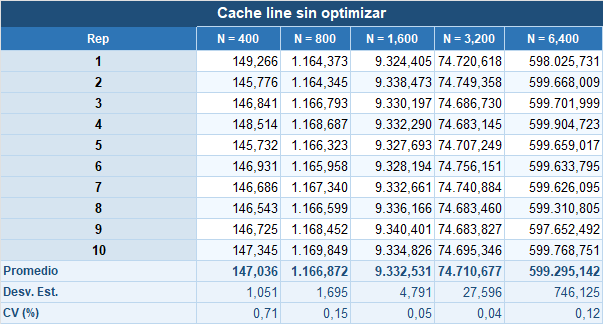
\includegraphics[width=0.8\textwidth]{images/tables/cache_noopt.png}
      \caption{Tiempos de ejecución del algoritmo secuencial optimizado por cache line para diferentes tamaños de matrices.}
      \label{fig:tiempos_cache}
\end{figure}

\begin{figure}[H]
   \centering
   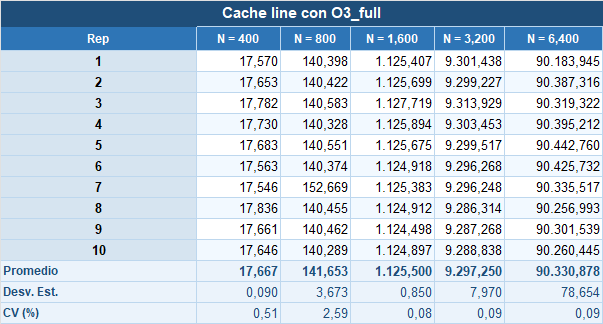
\includegraphics[width=1\textwidth]{images/tables/cache_opt.png}
   \caption{Tiempos de ejecución del algoritmo secuencial optimizado por cache line con optimizaciones.}
   \label{fig:tiempos_cache_opt}
\end{figure}

\begin{figure}[H]
   \centering
   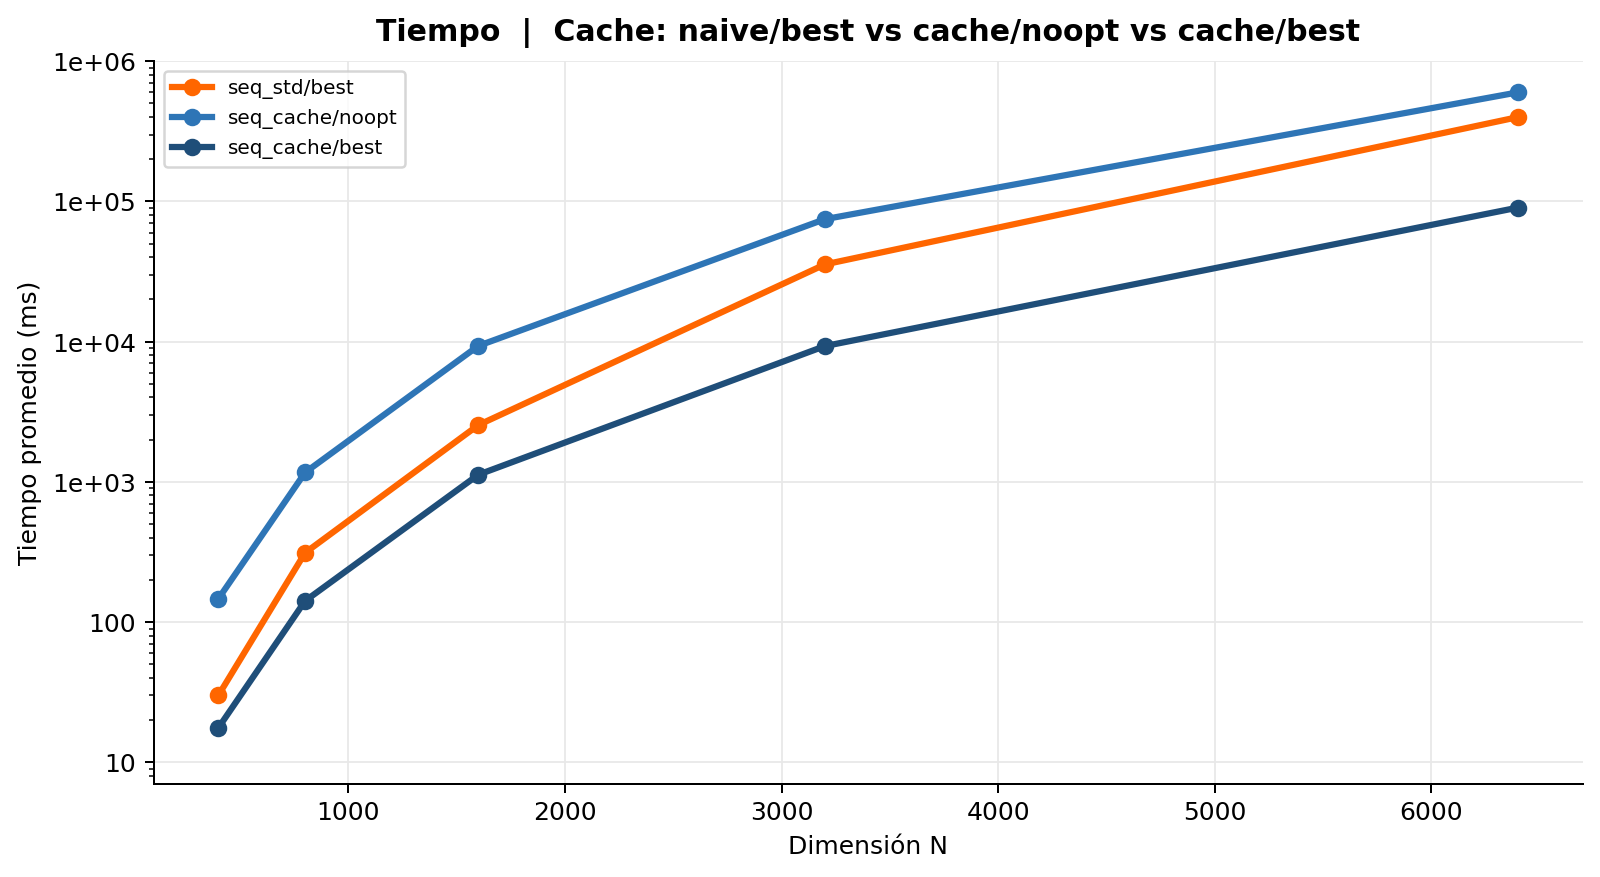
\includegraphics[width=1\textwidth]{images/charts/time_cache.png}
   \caption{Gráfica de tiempos de ejecución del algoritmo secuencial optimizado por cache line.}
   \label{fig:grafica_cache}
\end{figure}

\begin{figure}[H]
   \centering
   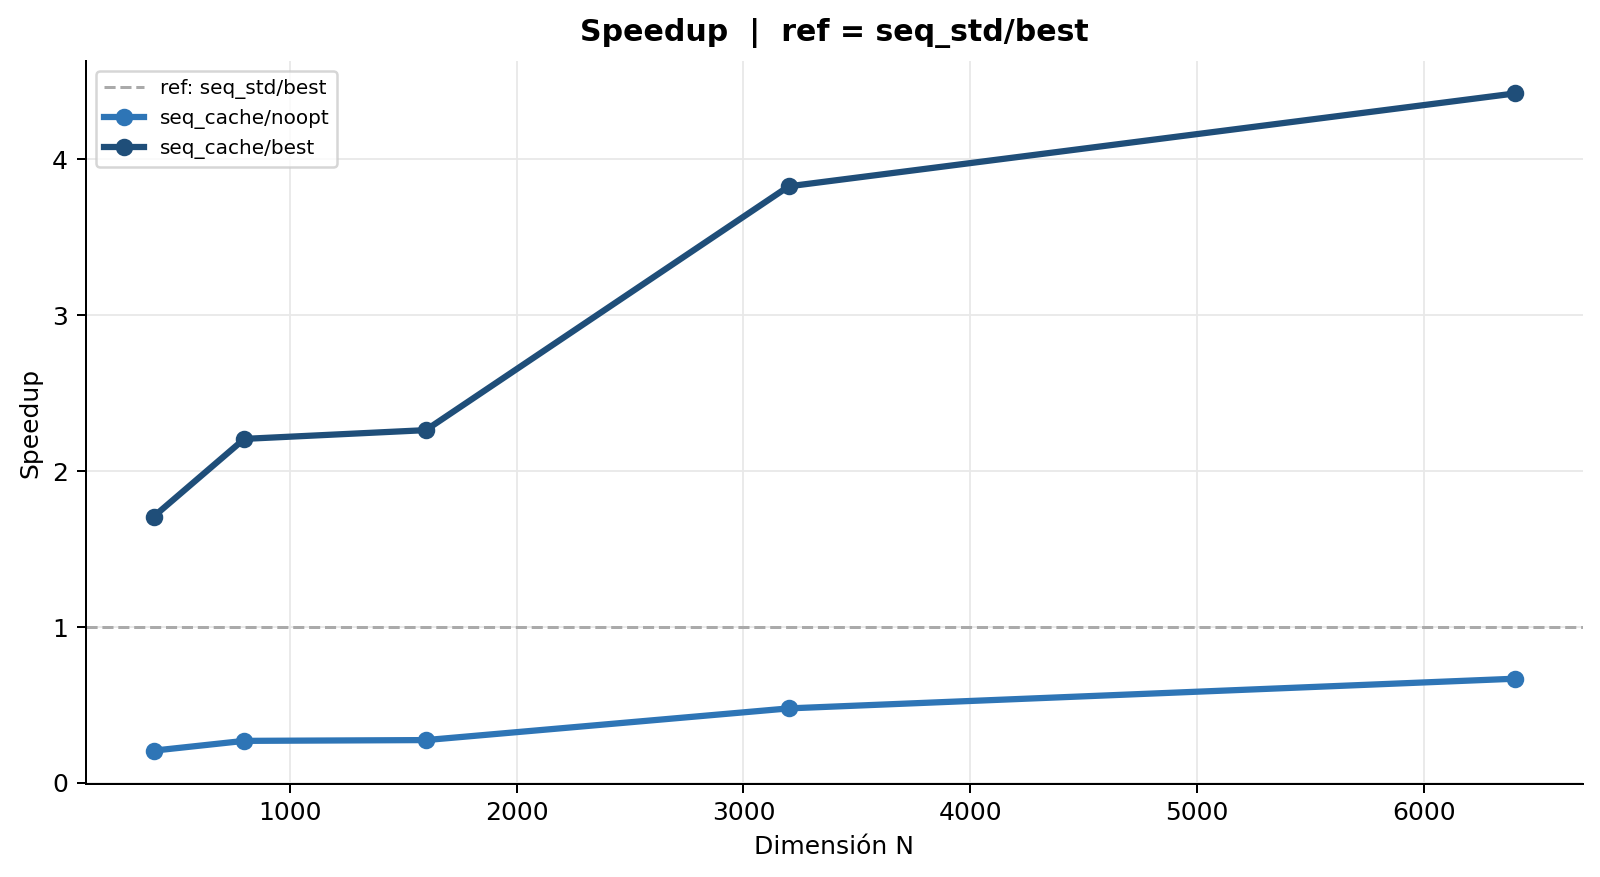
\includegraphics[width=1\textwidth]{images/charts/speedup_cache.png}
   \caption{Gráfica de Speedup del algoritmo secuencial optimizado por cache line.}
   \label{fig:speedup_cache}
\end{figure}

\begin{figure}[H]
   \centering
   
\includegraphics[width=1\textwidth]{images/tables/speedup_cache.png}
   \caption{Tabla de Speedup del algoritmo secuencial optimizado por cache line.}
   \label{fig:speedup_cache}
\end{figure}


Para este caso se puede observar que el algoritmo secuencial optimizado por cache line no muestra una mejora significativa en el tiempo de ejecución en comparación con el algoritmo secuencial con optimización por compilador. Sin embargo, el algoritmo optimizado por cache line con optimización por compilador muestra una mejora en el rendimiento, especialmente para tamaños de matrices más grandes, esto se puede obseer en la gráfica de Speedup, donde se aprecia una mejora en el rendimiento del algoritmo optimizado por cache line con optimización por compilador en comparación con el algoritmo secuencial con optimización por compilador. Esto sugiere que la optimización por cache line puede ser efectiva para mejorar el rendimiento del algoritmo de multiplicación de matrices, especialmente para tamaños de matrices más grandes.